\documentclass[11pt]{article}
\newif\ifreview
\ifdefined\FORREVIEW\reviewtrue\else\reviewfalse\fi
\newif\ifwithsupp
\ifdefined\WITHSUPP\withsupptrue\else\withsuppfalse\fi
\usepackage[margin=0.92in]{geometry}
\usepackage{microtype}
\usepackage{amsmath,amssymb}
\usepackage{graphicx}
\usepackage{booktabs}
\usepackage{tabularx}
\usepackage{array}
\usepackage{enumitem}
\usepackage{xcolor}
\usepackage{caption}
\usepackage{subcaption}
\usepackage{float}
\usepackage{hyperref}
\usepackage{url}
\usepackage{lineno}
\hypersetup{colorlinks=true,linkcolor=black,citecolor=black,urlcolor=blue,pdftitle={Policy-TD: Teacher-Distilled Runtime Control for Frozen Small Language Models},pdfauthor={Surya Teja Avvaru; Krishna Sai Pokala; Varun Kumar Reddy Dodda},pdfkeywords={frozen language models, runtime control, teacher distillation, selective prediction, abstention, verifier-guided inference, small language models}}
\captionsetup{font=small,labelfont=bf}
\setlist[itemize]{leftmargin=1.2em,itemsep=0.18em,topsep=0.2em}
\setlist[enumerate]{leftmargin=1.4em,itemsep=0.18em,topsep=0.2em}
\newcolumntype{Y}{>{\raggedright\arraybackslash}X}
\newcommand{\policytd}{Policy-TD}
\newcommand{\ccg}{\mathrm{CCG}}
\newcommand{\pp}{\mathrm{pp}}
\emergencystretch=3em
\ifreview\linenumbers\fi


\begin{document}

\begin{center}
{\LARGE\bfseries Policy-TD: Teacher-Distilled Runtime Control for Frozen Small Language Models\par}
\vspace{0.8em}
\begin{tabular}{@{}>{\centering\arraybackslash}p{0.30\textwidth}>{\centering\arraybackslash}p{0.30\textwidth}>{\centering\arraybackslash}p{0.36\textwidth}@{}}
\textbf{Surya Teja Avvaru} & \textbf{Krishna Sai Pokala} & \textbf{Varun Kumar Reddy Dodda}\\[-0.1em]
{\small\href{mailto:avvarusuryateja@gmail.com}{\texttt{avvarusuryateja@gmail.com}}} &
{\small\href{mailto:ok50250@umbc.edu}{\texttt{ok50250@umbc.edu}}} &
{\small\href{mailto:vdodda1@bowiestate.edu}{\texttt{vdodda1@bowiestate.edu}}}
\end{tabular}
\vspace{0.45em}

{\small Surya Teja Avvaru is an Independent Researcher and the corresponding author.}\\[-0.05em]
{\small Manuscript - August 2026}
\end{center}
\vspace{0.35em}

\begin{abstract}
Small language models are attractive for local, low-cost, and privacy-sensitive deployment, but an important class of failures occurs when a model commits to an answer despite insufficient or contradictory evidence. We study this as a runtime-control problem. \policytd{} leaves student weights frozen and distills teacher-audited trace states into a compact multi-head controller that predicts semantic diagnostics, an intervention gate, and one of six bounded actions: finalization, abstention, repair, rollback, grounded continuation, or ordinary continuation. Across three independently trained guide seeds and three frozen student models, internal heldout accuracy rises from 31.0\% to 47.1--47.3\%, with 145--147 helped cases and zero observed harmed cases; router-off returns performance to 31.0\%. External-style stress accuracy rises from 33.56\% to 37.63\% with 110 helped and zero observed harmed cases. Public external accuracy changes only from 18.67\% to 19.22\%; under the conservative setting, 26 cases are helped and 6 harmed. Among conservative behavior-changing interventions, help yield falls from 74.0\% internally to 4.8\% on public external evaluation, showing that transfer is limited by recoverability as well as by intervention targeting. Gains concentrate in missing-information and unknowable-answer families. The evidence therefore supports a narrow claim: decision-space adaptation can recover answer-commitment failures when the frozen generator retains recoverable competence, but it does not create missing model capability.
\end{abstract}

\noindent\textbf{Keywords:} frozen language models; runtime control; teacher distillation; selective prediction; abstention; verifier-guided inference; small language models.

\section{Introduction}
Small language models are increasingly useful when latency, cost, privacy, and local deployment matter. Their failures, however, are not always failures of generation capacity alone. In many practical cases, the damaging event is premature answer commitment: a model finalizes when it should abstain, repair a mismatched final answer, roll back an unsafe trajectory, or request a more grounded continuation. This motivates a different adaptation question. Can reliability be improved without updating the student model, by learning when a frozen model should be allowed to commit?

We answer this question through \emph{decision-space adaptation}. Instead of modifying parameters inside the student language model, \policytd{} learns an external runtime policy over typed intervention actions. A frozen student produces a trace or candidate answer. A compact controller observes the resulting runtime state and decides whether to accept the answer or apply a bounded operation. The learned object is not a new answer generator and not a scalar verifier alone; it is a typed policy that governs answer commitment around a frozen generator.

This framing is intentionally narrower than general reasoning enhancement. A runtime controller cannot create missing mathematical, scientific, or factual competence inside a weak frozen model. Its value lies in controlling states where the generator has produced, or can still produce, enough information for a bounded intervention to improve the final output. We therefore evaluate \policytd{} using paired helped/harmed accounting, router-off ablation, family-level mechanism analysis, and external transfer tests. This evaluation design separates strong matched-domain answer-commitment gains from the weaker and more domain-dependent behavior observed on public external benchmarks.

This paper makes three contributions. First, it formalizes decision-space adaptation as a runtime-control alternative to weight-space, prompt-space, and search-space adaptation. Second, it instantiates the idea as \policytd{}, a teacher-distilled multi-head controller with validated semantic labels, an intervention gate, and a six-action runtime policy. Third, it evaluates the controller with paired helped/harmed metrics across internal heldout, external-style stress, and public external benchmarks, showing strong internal gains, causal dependence on the runtime router, and an explicit transfer boundary.

The paper is organized around a falsifiable causal claim. If a frozen model's error is an answer-commitment error, then a controller that recognizes the unsafe commitment state should improve the final output without changing the model. If the error reflects missing generator competence, runtime control should have limited effect and may harm by intervening on a state it cannot repair. This framing yields four testable expectations. First, guided runtime should outperform the frozen baseline on matched commitment-error families. Second, router-off should remove that gain if behavior-changing routing is the cause. Third, improvements should concentrate in families where unsupported finalization is the dominant failure mode rather than appearing as a broad reasoning gain. Fourth, transfer should weaken as domain shift increases or as the frozen student loses the competence needed for a bounded intervention to recover the trajectory. The evaluation below tests all four expectations with paired outcomes.

\section{Related work and positioning}
\paragraph{Weight-space adaptation.} Fine-tuning, adapters, LoRA, and QLoRA adapt model behavior by updating parameters or adding trainable modules inside the model \cite{hu2021lora,dettmers2023qlora}. Instruction tuning and reinforcement learning from human feedback similarly alter the model or its learned policy \cite{ouyang2022training}. \policytd{} instead leaves the student weights fixed and learns only an external controller. The method is complementary to weight-space adaptation: it can be viewed as a reliability layer around a frozen generator rather than a replacement for model adaptation.

\paragraph{Prompt-space and search-space inference.} Chain-of-thought prompting, self-consistency, ReAct, and Tree of Thoughts improve performance by eliciting, sampling, or searching over model-generated reasoning trajectories \cite{wei2022chain,wang2022selfconsistency,yao2022react,yao2023tree}. Those methods change the inference path of the generator. \policytd{} changes the control decision around a generated trace: whether the current state should be finalized, answered with an abstention, repaired, rolled back, continued under a grounding constraint, or simply continued.

\paragraph{Runtime controllers for budgeted inference.} Recent work on bit-calibrated test-time scaling treats frozen quantized inference as a controllable runtime process, using lightweight online signals to decide whether a model should continue, stop, or escalate under a hard token budget \cite{patarlapalli2026bitcal}. \policytd{} shares the view that useful inference behavior can be governed outside the frozen backbone, but differs in its target: it distills teacher-audited semantic labels into a typed intervention policy for answer commitment rather than calibrating token-budget halting decisions.

\paragraph{Verifiers, feedback, and process supervision.} Outcome verifiers and process-supervision methods judge candidate reasoning or steps, especially for mathematical reasoning \cite{cobbe2021training,lightman2023lets}. Self-Refine and Reflexion use feedback loops to revise model outputs \cite{madaan2023selfrefine,shinn2023reflexion}; Constitutional AI and distilling step-by-step show that AI feedback and rationales can supervise downstream behavior \cite{bai2022constitutional,hsieh2023distilling}. \policytd{} shares the idea of teacher-provided supervision but differs in the unit of action. The controller does not merely score correctness or ask the model to reflect; it selects a typed runtime operation.

\paragraph{Selective prediction and abstention.} Selective classification formalizes the risk-coverage tradeoff of abstaining under uncertainty \cite{geifman2017selective}. SQuAD2 makes answerability explicit by requiring systems to avoid unsupported answers \cite{rajpurkar2018know}. \policytd{} generalizes abstention into a broader runtime action space. Abstention is one action, but the controller can also repair, roll back, or request a grounded continuation when the state is not simply unanswerable.

These strands motivate but do not subsume the present formulation. Weight-space methods change model parameters, prompt- and search-space methods change the inference trajectory, verifier-style methods score candidate outputs, and selective prediction decides whether to abstain. \policytd{} combines a subset of these ideas into a different unit of adaptation: a teacher-distilled, typed runtime policy over states produced by an unchanged student. This positioning is important for interpreting the evidence below. The method should succeed when the failure is unsafe commitment, but it should have limited effect when the frozen generator lacks the competence needed to produce a recoverable trajectory.

\begin{table}[H]
\centering
\small
\caption{\textbf{Adaptation axes for frozen small language models.} The contribution is not a new weight update or prompt-search recipe, but a learned runtime policy over answer-commitment decisions.}
\label{tab:axes}
\begin{tabularx}{\linewidth}{p{0.23\linewidth}Y Y Y}
\toprule
Axis & What changes & Learned object & Status of student model \\
\midrule
Weight-space adaptation & Parameters, adapters, or trainable modules & Updated weights or attached adapter & Modified \\
Prompt/search-space inference & Prompts, trajectories, samples, or search path & Generated reasoning/search trajectory & Frozen or unchanged \\
Decision-space adaptation & Runtime commitment decisions & Intervention gate and typed action policy & Frozen; weights unchanged \\
\bottomrule
\end{tabularx}
\end{table}

\section{Formalization and paired evaluation}\label{sec:formal}
Let \(S_W : \mathcal{X} \rightarrow \mathcal{Y}\) denote a frozen student language model with fixed weights \(W\). For prompt \(x_i\), the student emits a trace or response
\begin{equation}
    y_i = S_W(x_i),
\end{equation}
and an extraction function obtains a candidate final answer
\begin{equation}
    \hat{a}_i = E(y_i).
\end{equation}
The controller observes a runtime state
\begin{equation}
    z_i = \phi(x_i, y_i, \hat{a}_i, m_i),
\end{equation}
where \(m_i\) denotes optional task-contract metadata used for analysis or evaluation. Weight-space adaptation changes \(W\); decision-space adaptation keeps \(W\) fixed and learns controller parameters \(\theta\).

The action space is
\begin{equation}
\mathcal{U}=\{\texttt{finalize},\texttt{say\_unknown},\texttt{repair\_final},\texttt{rollback},\texttt{force\_grounded\_step},\texttt{continue}\}.
\end{equation}
We distinguish non-changing baseline actions from behavior-changing interventions,
\begin{equation}
\mathcal{U}_{\mathrm{base}}=\{\texttt{finalize},\texttt{continue}\},\qquad
\mathcal{U}_{\mathrm{change}}=\mathcal{U}\setminus\mathcal{U}_{\mathrm{base}}.
\end{equation}
The baseline action \(u_i^B\in\mathcal{U}_{\mathrm{base}}\) is the action the frozen student path would take without Policy-TD: finalization for terminal candidate answers and ordinary continuation for nonterminal states. This notation avoids treating \texttt{finalize} and \texttt{continue} as behavior-changing interventions.

A teacher audit maps runtime states to semantic and policy labels,
\begin{equation}
T(z_i)=(\ell_i^{\mathrm{sup}},\ell_i^{\mathrm{ans}},\ell_i^{\mathrm{ent}},\ell_i^{\mathrm{log}},\ell_i^{\mathrm{tr}},g_i^\star,u_i^\star),
\end{equation}
where semantic labels describe support, answerability, entity-state consistency, logical-operator consistency, and answer-trace consistency; \(g_i^\star\in\{0,1\}\) is the teacher intervention target; and \(u_i^\star\in\mathcal{U}\) is the best-action target. A schema validator \(V\) admits only valid teacher outputs,
\begin{equation}
V(T(z_i))=1,
\end{equation}
so malformed or off-schema teacher outputs are rejected rather than silently converted into fallback labels.

The guide is a multi-head controller,
\begin{equation}
C_\theta(z_i)=\left(p_\theta(\ell^1|z_i),\ldots,p_\theta(\ell^K|z_i),p_\theta(g|z_i),p_\theta(u|z_i)\right),
\end{equation}
trained with a weighted cross-entropy objective,
\begin{equation}
\mathcal{L}_{\mathrm{TD}}(\theta)=\sum_i\left[\sum_{k\in\mathcal{K}}\lambda_k\,\mathrm{CE}(\ell_i^k,p_\theta(\ell^k|z_i))+\lambda_g\,\mathrm{CE}(g_i^\star,p_\theta(g|z_i))+\lambda_u\,\mathrm{CE}(u_i^\star,p_\theta(u|z_i))\right].
\end{equation}
At inference time, the intervention gate is
\begin{equation}
\hat{g}_i=\mathbf{1}\left[p_\theta(g=1|z_i)\geq\tau_g\right].
\end{equation}
The selected action is
\begin{equation}
\hat{u}_i=
\begin{cases}
\arg\max_{u\in\mathcal{U}}p_\theta(u|z_i), & \hat{g}_i=1,\\
u_i^B, & \hat{g}_i=0.
\end{cases}
\end{equation}
A runtime executor maps the selected action to a guided output,
\begin{equation}
o_i^G=A_{\hat{u}_i}(x_i,y_i,\hat{a}_i,S_W),
\end{equation}
while the baseline output is
\begin{equation}
o_i^B=A_{u_i^B}(x_i,y_i,\hat{a}_i,S_W).
\end{equation}
Router-off sets \(\hat{u}_i=u_i^B\) for all examples, preserving the evaluation path while disabling behavior-changing actions.

Let \(J(x_i,o_i)\in\{0,1\}\) be the benchmark judge or scoring rule. Baseline and guided correctness are
\begin{equation}
b_i=J(x_i,o_i^B),\qquad q_i=J(x_i,o_i^G).
\end{equation}
The helped and harmed counts are
\begin{equation}
H=\sum_{i=1}^{N}\mathbf{1}[b_i=0\land q_i=1],\qquad
D=\sum_{i=1}^{N}\mathbf{1}[b_i=1\land q_i=0].
\end{equation}
We define commitment-control gain as the paired accuracy change,
\begin{equation}
\mathrm{CCG}_{\mathrm{pp}}=100\cdot\frac{H-D}{N}.
\end{equation}
This identity makes helped/harmed accounting the central paired reliability metric: average accuracy improves only when recovered baseline failures outnumber corrupted baseline successes.

For behavior-changing interventions, let
\begin{equation}
I=\sum_{i=1}^{N}\mathbf{1}[\hat{u}_i\in\mathcal{U}_{\mathrm{change}}],\qquad
T=\sum_{i=1}^{N}\mathbf{1}[\hat{u}_i\in\mathcal{U}_{\mathrm{change}}\land b_i=0].
\end{equation}
We report three distinct post-hoc diagnostics,
\begin{equation}
\mathrm{TP}_{\mathrm{int}}=\frac{T}{\max(I,1)},\qquad
\mathrm{HY}=\frac{H}{\max(I,1)},\qquad
\mathrm{DY}=\frac{D}{\max(I,1)}.
\end{equation}
Here \(\mathrm{TP}_{\mathrm{int}}\) is \emph{targeting precision}: the fraction of interventions that occur on baseline-incorrect rows. \(\mathrm{HY}\) is help yield, the fraction of interventions that actually recover a baseline failure, and \(\mathrm{DY}\) is harm yield, the fraction that corrupt a baseline success. Targeting precision is diagnostic only because baseline correctness is not known at deployment. Separating targeting from outcome yield is important: a controller may correctly identify a failing state yet still be unable to repair it when the frozen generator lacks recoverable competence.

For figure intervals, we use the paired row-level difference \(d_i=q_i-b_i\in\{-1,0,1\}\). The standard error for \(\mathrm{CCG}_{\mathrm{pp}}\) is estimated as
\begin{equation}
\mathrm{SE}=100\sqrt{\frac{1}{N(N-1)}\sum_{i=1}^{N}\left(d_i-\bar{d}\right)^2},
\end{equation}
with displayed 95\% intervals \(100\bar{d}\pm1.96\,\mathrm{SE}\). The interval is descriptive and paired; it is not an independent-sample comparison or a prompt-cluster generalization interval.

\section{Policy-TD controller design}
\subsection{Teacher-distilled tandem workflow}
\policytd{} separates four roles. The frozen student generates a trace or candidate answer. The teacher audits training traces offline using a strict schema. The guide learns to approximate the teacher's semantic and policy labels. The runtime controller converts guide predictions into an executable action. The evaluator or judge scores final outputs during heldout evaluation. This separation is important: teacher labels define the training target, but the primary endpoint is paired runtime behavior.


\begin{figure}[H]
    \centering
    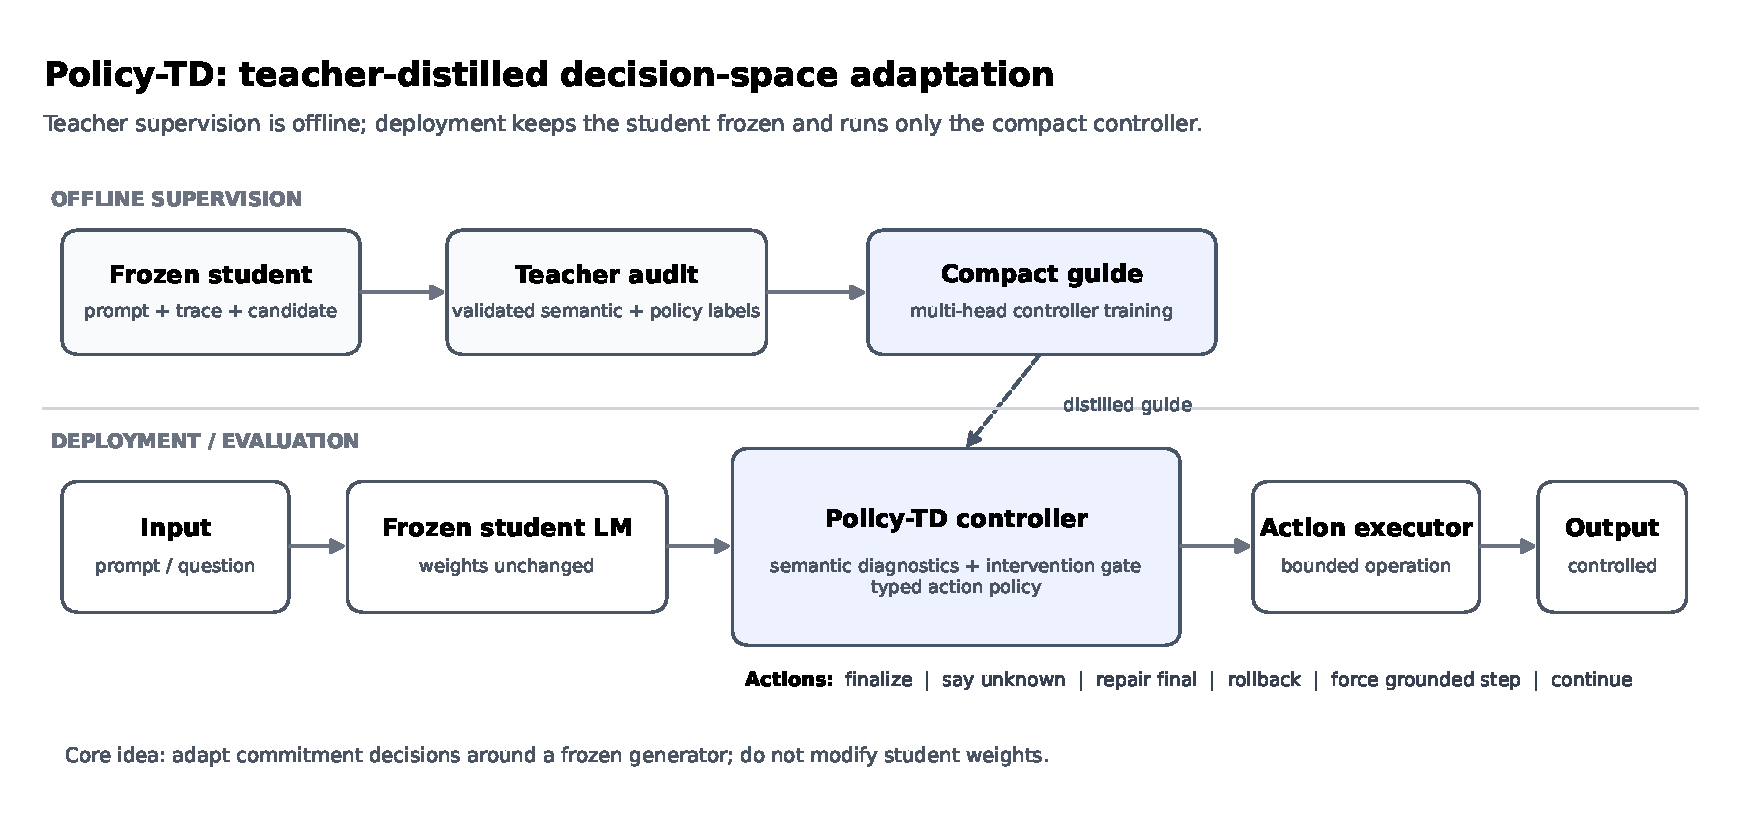
\includegraphics[width=0.98\linewidth]{figures/policy_td_architecture_final.pdf}
    \caption{\textbf{Policy-TD separates offline teacher supervision from runtime control.} The teacher audits frozen-student trace states only during supervision. Deployment uses the unchanged student plus the distilled compact guide, which combines semantic diagnostics, an intervention gate, and a typed action policy. The six actions are bounded: finalize, abstain, repair, rollback, force a grounded step, or continue.}
    \label{fig:architecture}
\end{figure}

The workflow is tandem rather than end-to-end generative. During supervision, the student and teacher operate together: the frozen student supplies the failure-prone trace state, while the stronger teacher labels what kind of failure is present and which bounded action should be taken. During deployment, the teacher is absent. The trained guide must infer the same intervention decision from the student's runtime state. This is why \policytd{} is a distillation method: teacher judgment is compressed into a small non-generative policy that can run alongside frozen students.

Offline, teacher-audited traces are converted into validated semantic and policy labels. The semantic labels describe what is wrong, if anything, with the trace. The policy labels describe whether an intervention should occur and which action should be selected. Online, the frozen student produces a trace, the guide predicts semantic heads and policy heads, and a conservative gate decides whether a behavior-changing action is allowed. If the gate blocks intervention, the system finalizes or continues without overriding the baseline trajectory. If the gate permits intervention, the action executor applies the selected typed operation.

This structure makes the gate the central risk-control mechanism. A high-recall gate can recover many baseline failures but risks corrupting correct answers. A very conservative gate reduces harms but leaves more baseline failures untouched. The conservative and higher-recall operating points should therefore be interpreted as different points on a gain-risk frontier, not as different student models.

Three design choices follow from this framing. First, the controller receives trace-state evidence rather than only a final answer string, because the correct action may depend on whether the trace supports, contradicts, or merely fails to justify the final answer. Second, semantic heads are trained alongside policy heads so that intervention decisions are tied to interpretable failure modes rather than to a single opaque risk score. Third, evaluation is paired against the frozen baseline because a runtime controller is useful only if it recovers failures without unnecessarily changing already-correct outputs.
\begin{table}[H]
\centering
\small
\caption{\textbf{Semantic heads, gate, and runtime policy.} The controller is trained to diagnose failure modes and select a bounded runtime operation.}
\label{tab:heads}
\begin{tabularx}{\linewidth}{p{0.20\linewidth}p{0.16\linewidth}Y Y}
\toprule
Signal & Type & Runtime role & Typical action linkage \\
\midrule
Claim support & Semantic head & Detects unsupported, contradicted, or weakly supported final claims & \texttt{say\_unknown}, \texttt{rollback}, \texttt{force\_grounded\_step} \\
Answerability & Semantic head & Detects prompts that lack sufficient information for a supported answer & \texttt{say\_unknown} \\
Entity/state consistency & Semantic head & Detects entity binding, state tracking, or transition errors & \texttt{rollback}, \texttt{force\_grounded\_step} \\
Logical-operator consistency & Semantic head & Detects quantifier, negation, and operator mismatches & \texttt{repair\_final}, \texttt{rollback} \\
Answer-trace consistency & Semantic head & Detects cases where the final answer disagrees with the trace & \texttt{repair\_final} \\
Should-intervene & Gate head & Decides whether ordinary finalization should be overridden & Enables or blocks behavior-changing action \\
Best action & Policy head & Selects the typed runtime operation & Six-action vocabulary \\
\bottomrule
\end{tabularx}
\end{table}

Table~\ref{tab:heads} is the practical interpretation of the formal controller. The semantic heads are not intended to be standalone benchmark labels; they are intermediate diagnostics used to make intervention decisions more structured. For example, an answerability failure should primarily route toward abstention, whereas an answer-trace mismatch can be repairable if the trace contains enough evidence. The \texttt{should-intervene} head is the conservative gate that decides whether these signals should actually change the output. The \texttt{best-action} head then chooses the operation to apply.

\begin{table}[H]
\centering
\small
\caption{\textbf{Runtime actions.} Actions are executable control decisions, not free-form answer labels.}
\label{tab:actions}
\begin{tabularx}{\linewidth}{p{0.24\linewidth}Y Y}
\toprule
Action & Runtime operation & Principal risk \\
\midrule
\texttt{finalize} & Accept the current candidate answer & Preserves an incorrect baseline if the gate misses a failure \\
\texttt{say\_unknown} & Abstain because the prompt lacks sufficient support & Can harm answerable examples if over-applied \\
\texttt{repair\_final} & Apply a bounded final-answer correction when trace evidence supports it & Can over-correct when the trace is unreliable \\
\texttt{rollback} & Discard an unsafe or unsupported trajectory & Can discard useful partial reasoning \\
\texttt{force\_grounded\_step} & Request a constrained continuation from the frozen student & Cannot repair missing model competence \\
\texttt{continue} & Permit ordinary continuation without immediate override & Can delay intervention if the state is already unsafe \\
\bottomrule
\end{tabularx}
\end{table}

The six actions are intentionally bounded. The controller is not allowed to synthesize an unconstrained new answer in the way a second language model might. Instead, it can accept the current answer, abstain, perform a bounded final-answer repair, discard an unsafe trajectory, request a grounded continuation, or permit ordinary continuation. This action vocabulary is what turns a verifier-like signal into a control policy: the system does not only ask whether the current answer is safe; it asks what should happen next.

\subsection{Guided inference algorithm}
\noindent\textbf{Algorithm 1: Policy-TD guided inference.}
\begin{enumerate}
    \item Input prompt \(x\), frozen student \(S_W\), controller \(C_\theta\), and gate threshold \(\tau_g\).
    \item Generate a student trace \(y=S_W(x)\) and extract a candidate final answer \(\hat{a}=E(y)\).
    \item Construct runtime state \(z=\phi(x,y,\hat{a},m)\).
    \item Predict semantic heads, gate probability \(p_\theta(g=1|z)\), and action distribution \(p_\theta(u|z)\).
    \item If router-off is enabled, return the baseline output.
    \item If \(p_\theta(g=1|z)<\tau_g\), return the baseline action \(u^B\) without behavior-changing intervention.
    \item Otherwise choose \(\hat{u}=\arg\max_{u\in\mathcal{U}}p_\theta(u|z)\).
    \item Execute \(o^G=A_{\hat{u}}(x,y,\hat{a},S_W)\) and return the guided output.
\end{enumerate}

Algorithm 1 clarifies the difference between \policytd{} and ordinary self-correction. The frozen student still supplies the candidate trajectory. The guide does not generate a replacement solution from scratch; it decides whether the trajectory should be trusted and which bounded operation should be applied. Router-off is therefore a meaningful causal ablation: it leaves the evaluation path intact but forces the gate closed, removing the behavior-changing component.

\section{Experimental design and implementation}
\subsection{Student models and guide architecture}
Experiments use three frozen student models: Qwen3-1.7B, SmolLM2-1.7B-Instruct, and TinyLlama-1.1B-Chat. Student models are not fine-tuned, adapter-tuned, or otherwise updated in the reported evaluations. This constraint is important because it makes the controller's contribution identifiable: any change in final behavior must come from the runtime policy rather than from altered student weights.

The guide is a compact encoder with multiple classification heads for semantic diagnostics and policy decisions. The shared representation receives the runtime state rather than only the final answer string, so the guide can compare the prompt, trace, and candidate final answer. The semantic heads predict support, answerability, entity-state consistency, logical-operator consistency, and answer-trace consistency. The policy heads predict should-intervene and best-action labels. This multi-head design is intended to make the intervention decision structured: semantic heads describe the failure mode; policy heads decide whether and how to act.

\subsection{Teacher-audited label construction}
Training traces are audited by a stronger GPT-family teacher model under a strict structured schema. The teacher is used only to create offline supervision for the guide; it is not present at deployment time and does not score the heldout outcomes. The teacher must emit labels from allowed vocabularies. Outputs with missing fields, invalid aliases, markdown, prose, or malformed structures are excluded or quarantined rather than coerced into defaults. This validation step is part of the method because silent fallback labels would contaminate the learned policy boundary. The teacher-label provenance is reported explicitly because the supervision source is part of the scientific claim: the heldout results test whether a compact guide can distill and operationalize those GPT-family audit labels without using the teacher model at inference time.

The audit schema serves two purposes. First, it decomposes a broad reliability judgment into learnable subdecisions: support, answerability, consistency, intervention, and action choice. Second, it prevents the guide from being trained on opaque free-form teacher prose. The guide therefore learns a typed intervention policy rather than a general instruction-following style. This is why exact best-action imitation is reported as diagnostic evidence, while runtime helped/harmed behavior remains the primary endpoint.


\subsection{Training and operating-point details}
The reported experiments used a DeBERTaV3-small encoder with mean pooling over the attention mask and separate linear classification heads for each semantic and policy target. In the guide-training stage used for the reported evaluations, the encoder is frozen and the classifier heads are trained with AdamW, batch size 4, maximum sequence length 512, learning rate \(5\times10^{-3}\), weight decay 0.01, and two epochs, with validation-loss checkpointing and learning-rate reduction on plateau. This training recipe reflects the intended role of the guide: it is a compact controller over structured trace-state labels, not a new language model.

The two guided operating points are reported by behavioral role. The \emph{conservative} operating point is the primary setting because it shows the best public-external gain-risk profile in the present evidence. The \emph{higher-recall diagnostic} operating point is included because it recovers additional public-external failures but also increases harmed cases. The distinction is important: the second setting is useful for analyzing the intervention frontier, not for claiming a safer default.

\subsection{Action executor and scoring rules}
The action executor applies bounded operations. \texttt{finalize} and \texttt{continue} preserve the baseline trajectory. \texttt{say\_unknown} returns a standardized abstention when the prompt is judged insufficiently supported. \texttt{repair\_final} requests a corrected final answer when the trace contains enough evidence but the final answer is mismatched. \texttt{rollback} discards a trajectory judged unsafe or unsupported and asks the frozen student for a constrained replacement final answer. \texttt{force\_grounded\_step} requests a continuation constrained to stated facts and necessary inference. Malformed guided outputs are rejected in favor of the baseline output rather than being counted as successful interventions.

Scoring is suite-specific but always paired. Internal prompts use the released gold answers and family contracts. SQuAD2-style answerable examples require a supported answer; SQuAD2-style unanswerable examples accept the standardized abstention when information is insufficient. ARC-Challenge examples are scored against the target answer choice after normalization. GSM8K examples are scored by the final numeric answer. In every case, the baseline and guided outputs are scored on the same prompt, student, and guide setting, making helped/harmed accounting well-defined.

\subsection{Evaluation suites}
The internal global heldout benchmark contains 100 prompts across ten families: answer-trace consistency, conservation, entity binding, missing information, quantifier/negation, state transition, style pressure, target lock, unknownability (unknowable-answer prompts), and unsupported assumption. It is disjoint from the training prompts of all three guide seeds. This suite is the primary controlled endpoint because it directly probes the answer-commitment failures the controller was designed to address.

The external-style stress suite contains 300 deterministic prompts designed to probe related abstention and harmful-change behavior under a shifted but still targeted distribution. The public external suite contains 400 examples from SQuAD2-style answerable QA, SQuAD2-style unanswerable QA, ARC-Challenge, and GSM8K. This suite is intentionally more heterogeneous: it tests whether the intervention policy transfers beyond the matched prompt families and where it fails. Each suite is evaluated across the relevant guide seeds and frozen students.

\subsection{Evaluation conditions and metrics}
The baseline condition evaluates the frozen student without behavior-changing \policytd{} intervention. The conservative operating point is the primary deployable setting reported in the paper. The higher-recall diagnostic operating point permits more interventions and is reported to expose the gain-risk frontier; it should not be read as uniformly safer. Router-off keeps the guide path present but disables behavior-changing actions by returning the baseline action \(u_i^B\). An oracle non-degradation condition appears only as a diagnostic upper bound in the supplementary material and is not treated as deployable.

We report baseline accuracy, guided accuracy, commitment-control gain, helped count, harmed count, intervention rate, post-hoc targeting precision, help yield, harm yield, unsupported-answer rate, and action distribution. The main paired reliability metric is helped/harmed accounting because it reveals whether the controller corrects baseline failures or corrupts baseline successes. Figure intervals use the paired row-level difference \(d_i=q_i-b_i\), defined in Section~\ref{sec:formal}; they are descriptive uncertainty intervals for the paired runtime effect, not independent-sample or prompt-cluster confidence intervals.

For a runtime controller, helped and harmed counts are more interpretable than accuracy alone. A controller with high average gain but many harmed cases may be unacceptable in a deployment setting; a controller with lower gain but zero observed harm may be preferable. Intervention rate is also not intrinsically good or bad. It is useful only when interventions are well targeted and the selected actions are actually recoverable by the frozen student. This is why the analysis separates targeting precision from help and harm yield in addition to reporting net gain.

\section{Results}
\subsection{RQ1: Does runtime control recover matched answer-commitment failures?}
The primary internal benchmark contains 100 globally held-out prompts across ten prompt families. It is disjoint from the training prompts of all three guide seeds. Each condition is evaluated across three guide seeds and three frozen students, giving 900 paired runtime rows for the internal suite. The external-style stress suite contains 300 deterministic stress prompts, producing 2700 rows. The public external benchmark contains 400 prompts spanning SQuAD2-style answerable QA, SQuAD2-style unanswerable QA, ARC-Challenge science QA, and GSM8K math word problems, producing 3600 rows. All results are paired at the runtime-row level.

Table~\ref{tab:primary} reports the main results. On the internal heldout, baseline accuracy is 31.0\%. \policytd{} improves accuracy to 47.11\% under the conservative operating point and 47.33\% under the higher-recall diagnostic operating point. The paired decomposition is 145 helped and zero harmed under the conservative operating point, and 147 helped and zero harmed under the higher-recall diagnostic operating point. Router-off returns accuracy to 31.0\%, with no helped or harmed cases, supporting the claim that improvements are caused by behavior-changing runtime routing rather than incidental changes in scoring or loading.

External-style stress transfer is positive with zero observed harmed cases: accuracy improves from 33.56\% to 37.63\%, with 110 helped and zero harmed cases under both the conservative and higher-recall operating points. Public external transfer is more limited. Pooled accuracy improves from 18.67\% to 19.22\%, but the conservative operating point produces 26 helped and 6 harmed cases, while the higher-recall diagnostic operating point produces 35 helped and 15 harmed cases. The result is therefore not a universal absence-of-harm claim; it is a distribution-dependent runtime-control result.

\begin{table}[H]
\centering
\scriptsize
\caption{\textbf{Primary paired runtime results.} Accuracy values are percentages. \(\Delta\) is commitment-control gain in percentage points. Helped means baseline incorrect and guided correct; harmed means baseline correct and guided incorrect. Router-off disables behavior-changing intervention.}
\label{tab:primary}
\begin{tabularx}{\linewidth}{p{0.21\linewidth}p{0.16\linewidth}rrrrrrr}
\toprule
Suite & Setting & N & Base & Guided & \(\Delta\) & Helped & Harmed & Int. rate \\
\midrule
Internal heldout & Router-off & 900 & 31.00 & 31.00 & 0.00 & 0 & 0 & 0.00 \\
Internal heldout & Conservative & 900 & 31.00 & 47.11 & 16.11 & 145 & 0 & 21.78 \\
Internal heldout & Higher-recall & 900 & 31.00 & 47.33 & 16.33 & 147 & 0 & 22.00 \\
External-style stress & Conservative & 2700 & 33.56 & 37.63 & 4.07 & 110 & 0 & 7.04 \\
External-style stress & Higher-recall & 2700 & 33.56 & 37.63 & 4.07 & 110 & 0 & 21.85 \\
Public external & Conservative & 3600 & 18.67 & 19.22 & 0.56 & 26 & 6 & 15.08 \\
Public external & Higher-recall & 3600 & 18.67 & 19.22 & 0.56 & 35 & 15 & 15.89 \\
\bottomrule
\end{tabularx}
\end{table}

\begin{table}[H]
\centering
\scriptsize
\caption{\textbf{Intervention-quality decomposition.} \(I\) is the number of behavior-changing interventions. Targeting precision is the post-hoc fraction of interventions applied to baseline-incorrect rows. Help and harm yields are the fractions of interventions that respectively recover a baseline failure or corrupt a baseline success.}
\label{tab:intervention_quality}
\begin{tabularx}{\linewidth}{p{0.23\linewidth}p{0.17\linewidth}rrrr}
\toprule
Suite & Setting & \(I\) & Targeting precision & Help yield & Harm yield \\
\midrule
Internal heldout & Conservative & 196 & 78.57\% & 73.98\% & 0.00\% \\
Internal heldout & Higher-recall & 198 & 78.79\% & 74.24\% & 0.00\% \\
External-style stress & Conservative & 190 & 84.21\% & 57.89\% & 0.00\% \\
External-style stress & Higher-recall & 590 & 94.92\% & 18.64\% & 0.00\% \\
Public external & Conservative & 543 & 88.95\% & 4.79\% & 1.10\% \\
Public external & Higher-recall & 572 & 87.94\% & 6.12\% & 2.62\% \\
\bottomrule
\end{tabularx}
\end{table}

The decomposition in Table~\ref{tab:intervention_quality} separates \emph{where} the controller intervenes from \emph{whether the bounded action succeeds}. Internally, the conservative controller makes 196 behavior-changing interventions; 154 target baseline-incorrect rows and 145 actually recover them, giving 78.57\% targeting precision and 73.98\% help yield with zero observed harm. On public external evaluation, targeting precision remains high at 88.95\%, but only 26 of 543 conservative interventions recover a baseline failure and 6 corrupt a baseline success. The corresponding help and harm yields are 4.79\% and 1.10\%. This distinction sharpens the transfer result: distribution shift does not merely make the gate less selective; it also leaves many correctly targeted failures unrecoverable by the available action executor and frozen generator.

The table should be read as a paired intervention study rather than as independent model comparisons. The baseline and guided outputs are evaluated on the same runtime rows, so every accuracy change decomposes into helped and harmed examples. On the internal heldout, the absence of observed harmed cases means the full gain comes from baseline-incorrect examples becoming correct. On public external evaluation, the positive pooled gain is much smaller and accompanied by harmed cases, indicating that the same gate is less selective under distribution shift.

Figure~\ref{fig:primary} visualizes these three facts. Panel a gives the average accuracy comparison, panel b shows the helped/harmed decomposition that reveals whether gains come from recovered failures or corrupted baseline successes, and panel c reports commitment-control gain as the paired net effect. The figure is intentionally empirical rather than schematic: it is meant to show that the core result is a runtime outcome difference, not a change to student weights or a prompt-format artifact.

\begin{figure}[H]
    \centering
    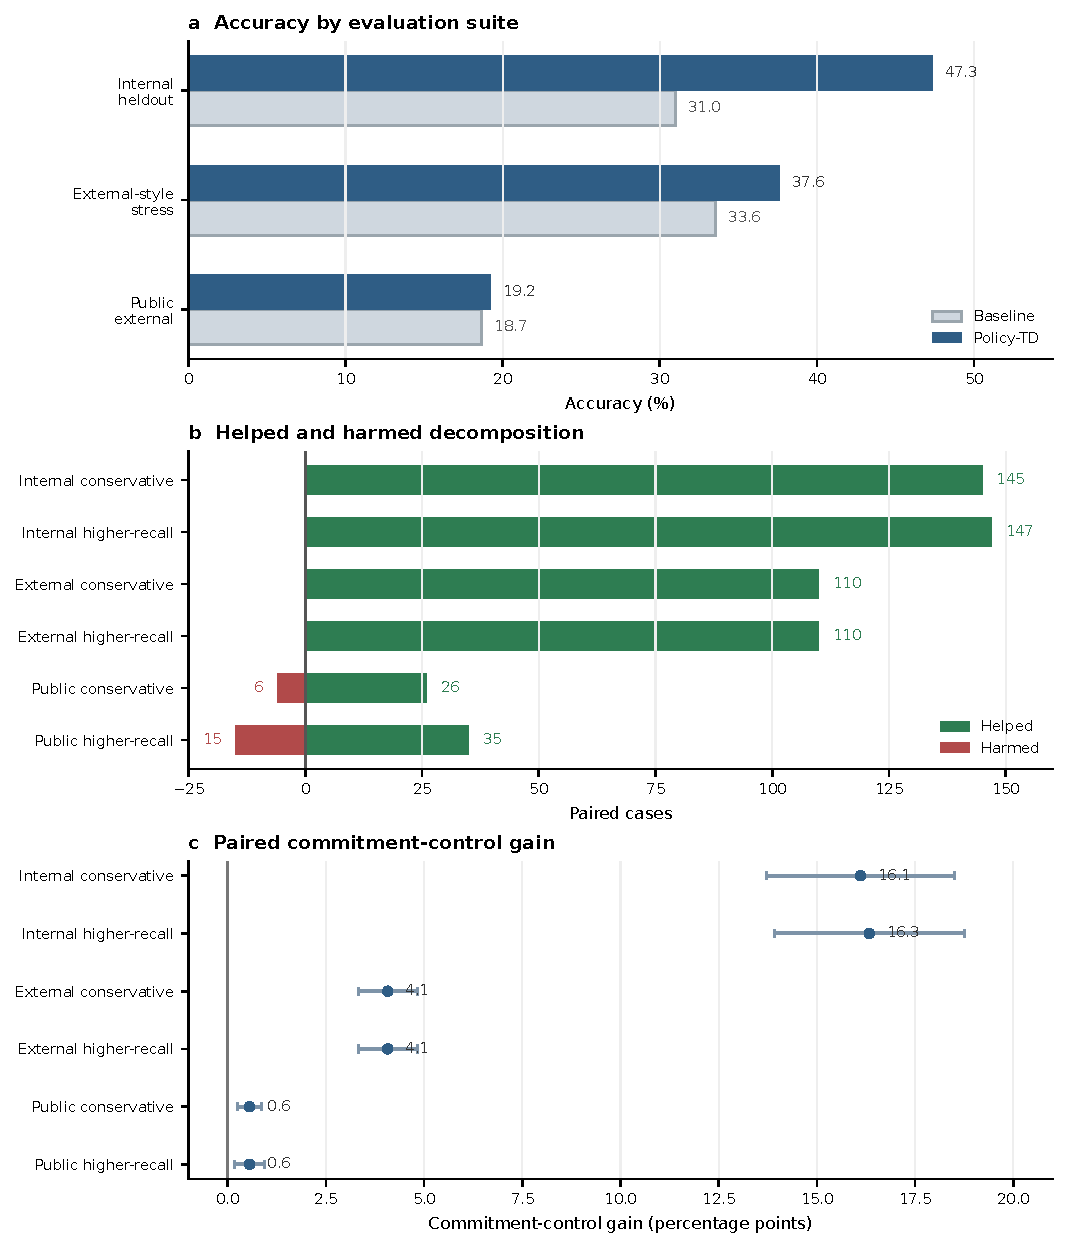
\includegraphics[width=0.98\linewidth]{figures/fig1_primary_results.pdf}
    \caption{\textbf{Primary runtime effect.} \textbf{a,} Baseline and guided accuracies are compared within each evaluation suite. The internal heldout shows a large matched-domain gain, external-style stress shows a smaller positive gain, and public external evaluation shows only modest transfer. \textbf{b,} The same result is decomposed into helped and harmed examples. This is the reliability-relevant view: a helped example is recovered by the controller, while a harmed example was correct under baseline and corrupted by guidance. \textbf{c,} Commitment-control gain summarizes the paired accuracy change, \(100(H-D)/N\). Intervals are descriptive paired normal approximations from trinary helped/harmed/unchanged runtime rows; because prompts recur across student/seed combinations, they are not prompt-cluster generalization intervals.}
    \label{fig:primary}
\end{figure}


\subsection{RQ2: Are gains localized to the intended failure mechanism?}
The internal effect is concentrated rather than diffuse. Missing-information prompts improve from 13.33\% baseline accuracy to 97.78\% under the conservative operating point and 100.0\% under the higher-recall diagnostic operating point. Unknownability prompts improve from 23.33\% to 100.0\% under both operating points. Most other internal families remain unchanged. This pattern is central to the interpretation of \policytd{}: the controller is not broadly increasing reasoning ability; it is changing the commitment behavior of the system in states where the frozen student would otherwise finalize despite insufficient, missing, or unknowable evidence.

The mechanism follows from the controller design. The semantic heads diagnose whether the trace state is supported, answerable, logically consistent, and aligned with the candidate final answer. The intervention gate then decides whether ordinary baseline behavior should be blocked, and the action head selects a bounded operation such as abstention, repair, rollback, grounded continuation, or ordinary continuation. Missing-information and unknownability families are therefore the expected high-gain region. Here, unknownability denotes prompts whose requested answer cannot be determined from the available evidence. In both families, the appropriate intervention is often to abstain or prevent unsupported finalization, not to solve a harder reasoning problem.

Figure~\ref{fig:mechanism} is the mechanism check. If \policytd{} were functioning as a general reasoning enhancer, gains would be expected across many prompt families, including families that require entity binding, quantifier handling, state tracking, or answer-trace consistency. Instead, nearly all internal gain appears in families whose dominant failure mode is unsafe answer commitment. This concentration supports a narrower and more defensible claim: \policytd{} improves selective reliability by governing when a frozen student is allowed to finalize.

The public external decomposition shows the corresponding boundary. The conservative operating point improves SQuAD2-style answerable QA by 1.11 percentage points, SQuAD2-style unanswerable QA by 0.67 points, and ARC-Challenge by 0.78 points, while GSM8K math decreases by 0.33 points. The higher-recall diagnostic operating point improves unanswerable QA more strongly but increases harms on answerable QA. These results are consistent with the same runtime-control interpretation. Answerability-sensitive QA transfers more favorably because the controller's labels and actions are aligned with support, answerability, and commitment decisions. GSM8K-style arithmetic transfers less favorably because many failures reflect missing symbolic or computational competence in the frozen generator, which a runtime gate cannot create.

The practical implication is that \policytd{} should be evaluated as a selective controller rather than as an all-purpose model improver. Its value is governed by two factors: intervention targeting and action recoverability. Behavior-changing actions should concentrate on baseline failures, but those failures must also be repairable by the frozen student and bounded executor. This is why paired helped/harmed analysis is not merely a reporting add-on; it is the mechanism-level metric. The internal result shows high commitment-control gain and high help yield with zero observed harmed cases, whereas public external transfer shows a much lower help yield and nonzero harm despite high post-hoc targeting precision. Together, these results define the present operating region of the method.

\begin{figure}[H]
    \centering
    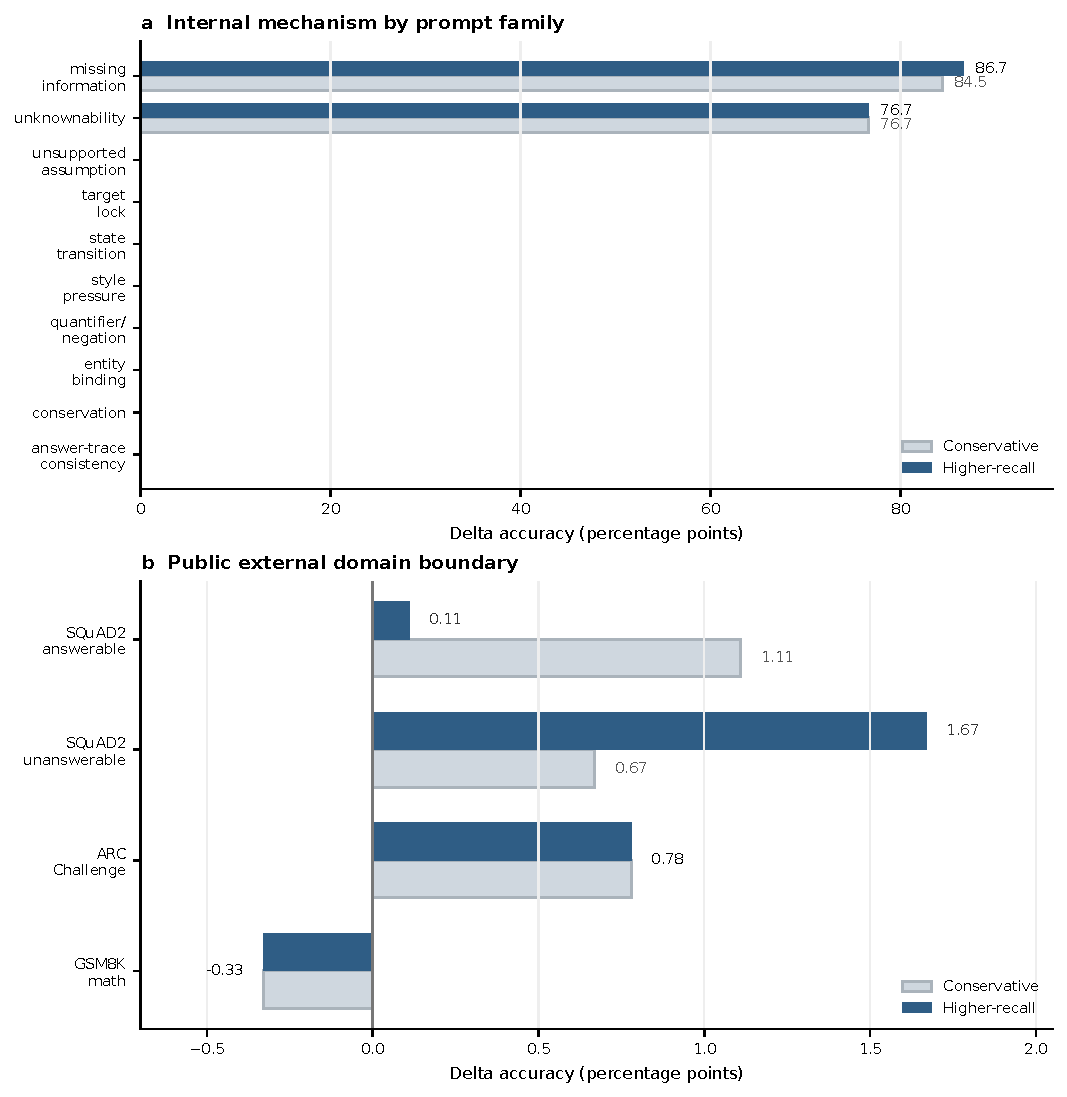
\includegraphics[width=0.98\linewidth]{figures/fig2_mechanism_boundary.pdf}
    \caption{\textbf{Mechanism and domain boundary.} \textbf{a,} Internal family-level effects are shown for both locked operating points. The gain is concentrated in missing-information and unknownability prompts, where the correct control decision is often to abstain or prevent unsupported finalization. The lack of broad movement in the other families supports a targeted answer-commitment mechanism rather than a general reasoning boost. \textbf{b,} Public external decomposition shows positive transfer on answerability-sensitive QA and ARC but not on GSM8K-style math. The higher-recall setting increases unanswerable-QA recovery but also exposes the risk of less selective intervention on answerable QA.}
    \label{fig:mechanism}
\end{figure}


\subsection{RQ3: What determines transfer under distribution shift?}
Student-level public external results expose a robustness boundary. Qwen3-1.7B gains 1.92 percentage points under both operating points. SmolLM2-1.7B gains 0.25 points under the conservative operating point and 0.50 points under the higher-recall diagnostic operating point. TinyLlama-1.1B loses 0.50 points under the conservative operating point and 0.75 points under the higher-recall setting, with harmed cases increasing when intervention is more aggressive. This boundary is informative rather than incidental: runtime control is most useful when the frozen generator retains enough latent competence for a bounded intervention to recover a failing trajectory.

The conservative operating point is therefore the more defensible deployable setting in the present evidence. The higher-recall diagnostic setting recovers more public external failures but also harms more baseline-correct cases. This is not a contradiction; it is the expected gain-risk tradeoff for a gated intervention system. Increasing intervention recall can recover additional baseline failures, but if the gate is less selective under distribution shift, it can also corrupt correct outputs.

Figure~\ref{fig:transfer} turns this limitation into an operating rule. The student-level panel shows that the controller transfers best when the frozen generator already has enough competence for a bounded intervention to matter. The helped/harmed panel shows that aggressive intervention can recover additional failures but also increases the risk of corrupting correct baseline answers. The practical implication is that guided mode should be validated per student-domain pair rather than assumed to transfer universally.

\begin{figure}[H]
    \centering
    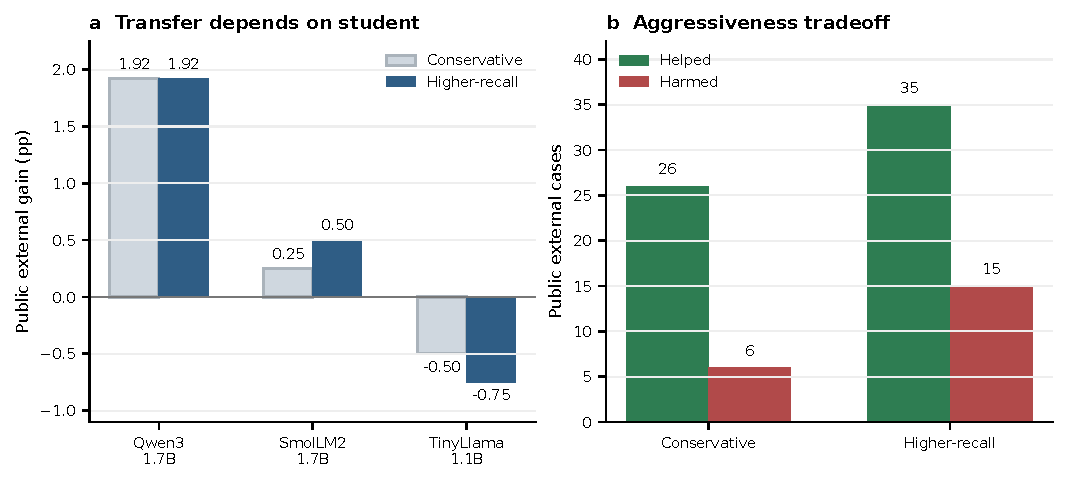
\includegraphics[width=0.98\linewidth]{figures/fig3_transfer_boundary.pdf}
    \caption{\textbf{Transfer boundary.} \textbf{a,} Public external transfer depends on the frozen student. Qwen3 shows positive transfer, SmolLM2 shows weak positive transfer, and TinyLlama shows negative transfer. This indicates that runtime control is not independent of generator competence. \textbf{b,} The higher-recall diagnostic setting recovers more public external failures than the conservative setting but also increases harmed cases. The result motivates a conservative deployment criterion: enable guided mode only when paired validation shows non-negative commitment-control gain and harmed cases remain within the tolerated threshold.}
    \label{fig:transfer}
\end{figure}

\section{Discussion and deployment boundary}
\policytd{} separates two questions that are often conflated: what a frozen generator is capable of producing, and whether the system should commit to the candidate it has produced. Parameter-efficient fine-tuning changes model competence by modifying trainable components inside the network. Prompt and search methods change how candidate trajectories are elicited. \policytd{} instead learns a bounded decision policy around an unchanged generator. The conceptual claim is therefore narrower than general model improvement: some errors can be corrected by controlling commitment even when the generator itself is not retrained.

The internal heldout evidence supports that narrow claim in three complementary ways. Accuracy improves substantially under both locked operating points, the gain is reproduced across three guide seeds and three frozen students, and router-off removes the gain while leaving the rest of the evaluation path intact. Mechanism analysis further localizes the effect: nearly all improvement occurs in missing-information and unknowable-answer families, while families dominated by other reasoning failures remain largely unchanged. Taken together, the evidence is more consistent with selective commitment control than with an unmeasured global increase in reasoning ability.

The external evidence is equally important because it defines where the mechanism stops working. External-style stress tests retain a positive effect with no observed harmed cases, but public external benchmarks show only a small pooled gain and nonzero harms. Qwen3 transfers positively, SmolLM2 only weakly, and TinyLlama negatively; GSM8K-style arithmetic also exposes a boundary. These failures are not incidental to the claim. They indicate that a controller cannot manufacture competence absent from the frozen generator, and that an intervention gate calibrated on one student-domain regime should not be assumed to remain selective after distribution shift. The intervention-quality decomposition adds a second distinction: even when interventions still concentrate on baseline-incorrect rows, the selected bounded action may fail to recover the example. Public conservative targeting precision is 88.95\%, yet help yield is only 4.79\%. This is evidence for a recoverability boundary, not only a gating boundary.

This suggests an operational deployment rule at the level of a student-domain pair \((S,D)\). Guided mode should be enabled only after paired validation shows
\begin{equation}
\mathrm{CCG}_{\mathrm{pp}}(S,D) \geq 0
\qquad\text{and}\qquad
D_{\mathrm{harm}}(S,D) \leq \delta,
\end{equation}
where \(D_{\mathrm{harm}}\) is the observed number of baseline-correct cases corrupted by guidance and \(\delta\) is the tolerated harm threshold. A strict operating policy sets \(\delta=0\). This is an empirical admissibility rule, not a safety guarantee: its purpose is to force deployment decisions to use the same paired unit on which controller value is measured rather than relying on average accuracy alone.

The next research step is therefore not simply to make the gate more aggressive. Stronger evidence would come from testing whether the same decision-space formulation survives changes in teacher source, guide architecture, student family and scale, domain, and action executor while preserving paired non-degradation behavior. Runtime overhead and calibration cost should also be measured explicitly. Such tests would distinguish a generally reusable control layer from a controller whose success depends on a narrow interaction between the present labels, students, and benchmark families.

\section{Limitations and validity}
\textbf{Construct validity.} The strongest result is measured on a custom internal heldout benchmark deliberately built around answer-commitment failure families. The split is global across all three guide seeds, but the benchmark still reflects the problem formulation and does not by itself establish broad language-model reliability.

\textbf{External validity.} The external-style stress suite is deterministic and remains close to the targeted failure regime, so it should be interpreted as shifted stress evidence rather than as fully independent public validation. Public external transfer is modest, model-dependent, and includes harmed cases. The present evidence therefore supports conditional transfer, not universal generalization.

\textbf{Supervision and measurement.} Teacher labels come from a stronger GPT-family model and can inherit teacher bias, inconsistency, or blind spots. Schema validation prevents malformed supervision from being silently accepted, but it cannot establish semantic correctness. Exact best-action transfer is therefore treated as diagnostic evidence; paired runtime outcomes remain the primary endpoint. Judge and audit samples are finite and may miss rare failure modes.

\textbf{Statistical and implementation scope.} The reported study covers three guide seeds, three frozen student models, two guided operating points, and a fixed compact guide architecture. The paired intervals describe uncertainty in the observed runtime-row effects. Because prompts are repeated across student and guide-seed combinations, those rows are not independent prompt draws; the intervals are descriptive and should not be interpreted as prompt-cluster generalization intervals. They are not evidence that the same effect will hold for arbitrary students, domains, controller architectures, or deployment conditions. Runtime latency and resource overhead are not yet a primary evaluated endpoint.

\textbf{Safety interpretation.} Zero observed harmed cases on the internal heldout and external-style stress suites is an empirical observation, not a correctness guarantee or a proof of safety. The public external results demonstrate that harms can emerge after distribution shift. \policytd{} should therefore be treated as a targeted decision-space adaptation method for answer-commitment control, with student-domain validation required before guided deployment.


\textbf{Reproducibility scope.} The public repository is intentionally curated rather than a complete export of the internal experimental workbench. It supports inspection of the method contract, frozen summary evidence, manifests, and verification logic, but it does not include every provider-specific teacher call, raw trace, local orchestration script, exploratory run, or unreleased checkpoint. Full from-scratch re-execution therefore requires additional runtime assets beyond the Git repository.
\section{Reproducibility, responsible release, and ethics}
\policytd{} is intended as a reliability layer for frozen small models, not as a correctness or safety guarantee. The paper reports harmed cases under public external transfer and recommends paired validation before enabling guided mode for a new student-domain pair. Diagnostic oracle conditions are separated from deployable settings, and negative transfer is reported as part of the method boundary.

The public repository at \url{https://github.com/suryaavvaru/policy-td} is a curated research artifact. It contains the stable action and label contracts, schema validation utilities, paired evaluation metrics, benchmark reports, frozen summary tables and provenance manifests, unit tests, documentation, and release-check scripts. Provider-specific teacher transcripts or credentials, large raw trace directories, local exploratory workbench scripts, and unreleased checkpoints are intentionally excluded. The release therefore supports artifact inspection, arithmetic verification, and traceability of the reported aggregate evidence; exact from-scratch replay of all original runs additionally requires the frozen runtime or checkpoint assets used during experimentation. Stable hashes for released assets are recorded in the release manifests.

\section{Conclusion}
\policytd{} tests a narrow proposition: some failures of a frozen language model are failures of answer commitment rather than failures of generator competence. A teacher-distilled external controller can recover a substantial fraction of those matched failures without changing student weights. On the internal heldout, accuracy rises from 31.0\% to 47.1--47.3\%, router-off removes the gain, and the effect is concentrated in missing-information and unknownability families. External-style stress retains a positive effect, while public external transfer is small, model-dependent, and includes harms. The intervention decomposition shows why this boundary matters: on public external data the controller often still targets baseline-incorrect states, but the bounded action rarely repairs them. Decision-space adaptation is therefore best understood as conditional runtime control around a frozen generator, not as a substitute for missing model capability. Future work should test the same formulation across stronger students, broader domains, alternative teacher sources and controller architectures, and explicit latency/cost measurements, with prompt-cluster uncertainty and calibration-frontier analysis where raw evaluation data permit them.

\section*{Author contributions}
Approximate contribution shares for this manuscript are Surya Teja Avvaru 75\%, Krishna Sai Pokala 15\%, and Varun Kumar Reddy Dodda 10\%. Surya Teja Avvaru is the principal contributor, and author order reflects relative contribution.

{\small
\begin{thebibliography}{99}
\bibitem{hu2021lora} Hu, E. J. et al. LoRA: Low-Rank Adaptation of Large Language Models. arXiv:2106.09685, 2021.
\bibitem{dettmers2023qlora} Dettmers, T. et al. QLoRA: Efficient Finetuning of Quantized LLMs. arXiv:2305.14314, 2023.
\bibitem{ouyang2022training} Ouyang, L. et al. Training language models to follow instructions with human feedback. arXiv:2203.02155, 2022.
\bibitem{wei2022chain} Wei, J. et al. Chain-of-Thought Prompting Elicits Reasoning in Large Language Models. arXiv:2201.11903, 2022.
\bibitem{wang2022selfconsistency} Wang, X. et al. Self-Consistency Improves Chain of Thought Reasoning in Language Models. arXiv:2203.11171, 2022.
\bibitem{yao2022react} Yao, S. et al. ReAct: Synergizing Reasoning and Acting in Language Models. arXiv:2210.03629, 2022.
\bibitem{yao2023tree} Yao, S. et al. Tree of Thoughts: Deliberate Problem Solving with Large Language Models. arXiv:2305.10601, 2023.
\bibitem{cobbe2021training} Cobbe, K. et al. Training Verifiers to Solve Math Word Problems. arXiv:2110.14168, 2021.
\bibitem{lightman2023lets} Lightman, H. et al. Let's Verify Step by Step. arXiv:2305.20050, 2023.
\bibitem{madaan2023selfrefine} Madaan, A. et al. Self-Refine: Iterative Refinement with Self-Feedback. arXiv:2303.17651, 2023.
\bibitem{shinn2023reflexion} Shinn, N. et al. Reflexion: Language Agents with Verbal Reinforcement Learning. arXiv:2303.11366, 2023.
\bibitem{bai2022constitutional} Bai, Y. et al. Constitutional AI: Harmlessness from AI Feedback. arXiv:2212.08073, 2022.
\bibitem{hsieh2023distilling} Hsieh, C.-Y. et al. Distilling Step-by-Step! Outperforming Larger Language Models with Less Training Data and Smaller Model Sizes. arXiv:2305.02301, 2023.
\bibitem{geifman2017selective} Geifman, Y. and El-Yaniv, R. Selective classification for deep neural networks. arXiv:1705.08500, 2017.
\bibitem{rajpurkar2018know} Rajpurkar, P., Jia, R., and Liang, P. Know What You Don't Know: Unanswerable Questions for SQuAD. arXiv:1806.03822, 2018.
\bibitem{he2021debertav3} He, P., Gao, J., and Chen, W. DeBERTaV3: Improving DeBERTa using ELECTRA-Style Pre-Training with Gradient-Disentangled Embedding Sharing. arXiv:2111.09543, 2021.
\bibitem{yang2025qwen3} Yang, A. et al. Qwen3 Technical Report. arXiv:2505.09388, 2025.
\bibitem{zhang2024tinyllama} Zhang, P., Zeng, G., Wang, T., and Lu, W. TinyLlama: An Open-Source Small Language Model. arXiv:2401.02385, 2024.
\bibitem{allal2024smollm} Allal, L. B. et al. SmolLM: Small language models and datasets. Hugging Face technical report/model release, 2024.
\bibitem{patarlapalli2026bitcal} Patarlapalli, S. B. and Avvaru, S. T. BitCal-TTS: Bit-Calibrated Test-Time Scaling for Quantized Reasoning Models. arXiv:2605.05561, 2026.
\bibitem{clark2018arc} Clark, P. et al. Think you have Solved Question Answering? Try ARC, the AI2 Reasoning Challenge. arXiv:1803.05457, 2018.
\end{thebibliography}
}

\end{document}
